\section{Key Technical Mechanisms}
\label{sec:mechanisms}

\subsection{Duplicate-Suppression Idempotency}

TradingView and similar platforms may retry webhook delivery after timeouts. Without deduplication, duplicate submissions can produce double positions. \textsc{HOOX} implements \emph{at-most-once acceptance} at the gateway within a configurable TTL; formal exactly-once semantics are not claimed across the full pipeline because Queues deliver at-least-once and the gateway fails open when the Durable Object is unavailable. The chosen design is a deliberate trade-off between availability and strict deduplication and is described in the threat model (Appendix~\ref{app:threat}).

\paragraph{Gateway mutex.} The \texttt{IdempotencyStore} Durable Object implements an atomic check-and-store operation using \texttt{blockConcurrencyWhile}, guaranteeing that concurrent requests for the same key cannot interleave between read and write (Algorithm~\ref{alg:idempotency}). Entries expire after a default TTL of 300\,s; alarm-based cleanup reclaims storage. Strongly consistent single-threaded objects with SQLite-backed storage are a common primitive in modern edge and serverless systems for serializing operations that would otherwise race~\cite{cloudflare-durable-objects,shahrad2020serverless}.

\begin{figure}[!htbp]
  \centering
  \begin{minipage}{0.92\linewidth}
  \textbf{Algorithm 1:} Idempotency check in \texttt{IdempotencyStore}
  \label{alg:idempotency}
  \small
  \begin{lstlisting}
Input:  key k, TTL tau
Output: true if new; false if duplicate
enter blockConcurrencyWhile
  e <- storage.get(k)
  if e != null and (now - e.storedAt) < tau then
    return false  // duplicate within TTL
  storage.put(k, {storedAt: now})
  schedule alarm at now + tau
  return true
  \end{lstlisting}
  \end{minipage}
\end{figure}

\paragraph{Semantics and limitations.}
\begin{itemize}
  \item \textbf{Key granularity:} The key excludes \texttt{requestId} and timestamp. Two legitimate signals with identical exchange, symbol, action, and quantity within the TTL window are treated as duplicates---a deliberate trade-off favoring retry safety over rapid scale-in.
  \item \textbf{Fail-open:} If the Durable Object RPC fails, the gateway permits the trade rather than halting execution---availability over strict deduplication.
  \item \textbf{Probe mode:} Synthetic requests with \texttt{probe: true} bypass idempotency and short-circuit in \texttt{trade-worker} before exchange validation, enabling repeatable internal latency measurement without side effects.
\end{itemize}

Listing~\ref{lst:idempotency-store} shows the production \texttt{IdempotencyStore} implementation (full source in Appendix~\ref{app:listings}); Listing~\ref{lst:probe-short-circuit} shows how synthetic probes bypass exchange submission for latency measurement. A second Durable Object class, \texttt{ExchangeConnectionManager}, maintains optional persistent WebSocket sessions per exchange for connection amortization; it does not currently participate in idempotency. Planned work includes exchange-native deduplication via \texttt{newClientOrderId} / \texttt{orderLinkId} fields derived from \texttt{requestId}.

\hooxsnippet{lst:idempotency-key}{idempotency-key.ts}{Idempotency key generation and fail-open DO check}
\hooxlisting{lst:probe-short-circuit}{probe-short-circuit.ts}{Probe short-circuit in \texttt{trade-worker} (no exchange call)}

\subsection{Gateway Hot Path}

The \texttt{hoox} \texttt{/webhook} handler minimizes serial I/O on the critical path. After a 100\,KB payload size guard, three security checks---kill switch, IP allow-list, and API key binding---execute in parallel via \texttt{Promise.all} (Listing~\ref{lst:webhook-parallel-checks}). Session creation and per-session rate limiting follow sequentially because they depend on the validated API key.

Validated trade payloads are schema-checked with \texttt{validateJson(WebhookPayloadSchema)} before dispatch. Trade and Telegram notification branches run concurrently when both are present in the same webhook.

\hooxsnippet{lst:webhook-parallel-checks}{webhook-parallel-checks.ts}{Parallel gateway pre-flight checks}

Internal routes between Workers authenticate with \texttt{X-Internal-Auth-Key} and constant-time comparison (Listing~\ref{lst:require-internal-auth}). The gateway fails closed when the binding is unconfigured; idempotency alone fails open on Durable Object errors (Section~\ref{sec:mechanisms}, duplicate-suppression paragraph).

\hooxsnippet{lst:require-internal-auth}{require-internal-auth.ts}{Internal service-to-service authentication}

\paragraph{Payload validation.} All trade payloads pass \texttt{validateJson(WebhookPayloadSchema)} before dispatch. The shared helper returns structured Zod path errors rather than throwing (Listing~\ref{lst:validate-json}).

\hooxsnippet{lst:validate-json}{validate-json.ts}{Zod-based request validation}

\paragraph{Service Binding transport.} Internal Worker calls use \texttt{serviceFetch}, which addresses bindings as \texttt{http://internal\{path\}} with a 30\,s \texttt{AbortSignal} timeout (Listing~\ref{lst:service-fetch}). Queue producers serialize a minimal trade envelope (Listing~\ref{lst:send-trade-to-queue}).

\hooxsnippet{lst:service-fetch}{service-fetch.ts}{Service Binding fetch with timeout}
\hooxsnippet{lst:send-trade-to-queue}{send-trade-to-queue.ts}{Queue producer message envelope}

\subsection{Smart Placement}

Latency-sensitive Workers---including \texttt{hoox}, \texttt{trade-worker}, \texttt{d1-worker}, and \texttt{agent-worker}---enable Smart Placement via \texttt{"placement": \{"mode": "smart"\}} in \texttt{wrangler.jsonc}. Cloudflare continuously measures RTT from its PoPs to a Worker's outbound origins (the exchange REST endpoints) and migrates isolate execution to a PoP that minimizes that RTT. The \texttt{dashboard} Worker intentionally disables Smart Placement to optimize for end-user browser proximity rather than exchange proximity.

\paragraph{Mechanism summary.} The dominant term for a signed REST order is the \emph{outbound} TLS+HTTP round-trip from the executing isolate to the exchange API origin. A VPS fixed in Virginia talking to a Tokyo or Singapore exchange incurs 80--200\,ms of public-internet RTT on that leg alone. Smart Placement places the \texttt{trade-worker} isolate in (or routes its outbound through) a PoP whose peering to that specific exchange endpoint is excellent (often single-digit milliseconds). Invocation routing (anycast + Smart Placement decision) is paid once per isolate lifecycle or migration; Workers cold starts are sub-3\,ms and isolates are kept warm across many PoPs. For a stream of signals the per-trade marginal cost is dominated by the optimized outbound leg, not the placement decision. Internal Service Bindings between \texttt{hoox} and \texttt{trade-worker} traverse Cloudflare's private fabric (not the public internet) and are sub-millisecond even when the two Workers execute in different PoPs. CDN-style proximity routing of this form has well-understood performance characteristics for general web traffic~\cite{nygren2010akamai,singh2015jupiter} and is applied here to a financial control plane.

The numbers in Table~\ref{tab:scenarios} therefore measure \emph{exchange API RTT originating from an optimally placed isolate}, not the cost to reach the first Cloudflare PoP. See Section~\ref{sec:evaluation} for the measurement methodology and caveats.

\subsection{Queue-Based Resilience}

The \texttt{trade-execution} queue decouples ingestion from execution. \texttt{hoox} acts as producer; \texttt{trade-worker} consumes with platform-level \texttt{max\_retries = 3} and application-level retries of five attempts with backoff $[0, 30, 60, 300, 900]$\,s. A dead-letter queue (\texttt{trade-execution-dlq}) captures permanently failed messages. Queue mode is KV-configurable (Table~\ref{tab:queue-modes}).

\paragraph{Producer routing.} \texttt{processTrade} (Listing~\ref{lst:process-trade}; full source in Appendix~\ref{app:listings}) selects among three modes: always direct Service Binding (\texttt{queue\_disabled}), direct-first with queue fallback (\texttt{queue\_failover}, default), or always enqueue (\texttt{queue\_everywhere}). Mode resolution reads \texttt{webhook:queue\_mode} from CONFIG\_KV with a 60\,s in-isolate cache (Listing~\ref{lst:get-queue-mode}).

\hooxsnippet{lst:get-queue-mode}{get-queue-mode.ts}{KV-backed queue mode with 60s cache}

\paragraph{Consumer retries.} The shared \texttt{createQueueHandler} (Listing~\ref{lst:queue-handler}; full source in Appendix~\ref{app:listings}) unifies retry semantics across Workers. \texttt{trade-worker} wires it with DLQ logging to D1 and Telegram notification on permanent failure (Listing~\ref{lst:trade-queue-consumer}).

\hooxsnippet{lst:trade-queue-consumer}{trade-queue-consumer.ts}{\texttt{trade-worker} queue consumer}

During exchange maintenance, queued signals eventually succeed in 99.97\% of cases within five minutes (Section~\ref{sec:evaluation}), at the cost of higher perceived latency when \texttt{queue\_everywhere} is enabled.

\subsection{Multi-Exchange Execution}

\texttt{trade-worker} routes orders through a provider-composed \texttt{ExchangeRouter}. KV table \texttt{routing:trade} can override the payload's declared exchange per symbol; per-exchange \texttt{enabled} and \texttt{use\_websocket} toggles gate runtime behavior without redeployment. The full \texttt{ExchangeRouter} is reproduced in Appendix~\ref{app:listings} (Listing~\ref{lst:exchange-router}).

After routing, \texttt{executeTrade} applies KV risk limits (kill switch, default leverage, max position size), optionally sets leverage, and dispatches \texttt{LONG}/\texttt{SHORT}/\texttt{CLOSE\_*} actions via exchange-specific HMAC clients. The risk gate and REST placement path are reproduced in Appendix~\ref{app:listings} (Listing~\ref{lst:execute-trade-risk}); WebSocket execution via \texttt{ExchangeConnectionManager} is selected when KV enables \texttt{use\_websocket}.

\paragraph{HMAC signing.} Exchange REST clients extend \texttt{BaseExchangeClient}, which imports the API secret as a \texttt{CryptoKey} once per isolate and signs query strings with HMAC-SHA256 via \texttt{crypto.subtle} (Listing~\ref{lst:crypto-sign}). The Binance futures client appends \texttt{timestamp} and \texttt{signature} query parameters per the exchange specification; the full authenticated request construction is in Appendix~\ref{app:listings}.

\hooxsnippet{lst:crypto-sign}{crypto-sign.ts}{Shared HMAC-SHA256 signing primitive}

Figure~\ref{fig:signal-lifecycle} summarizes the end-to-end synchronous path; queued modes defer steps 3--4 until consumer pickup.

\begin{figure}[!htbp]
  \centering
  \IfFileExists{figures/signal-lifecycle.pdf}{%
    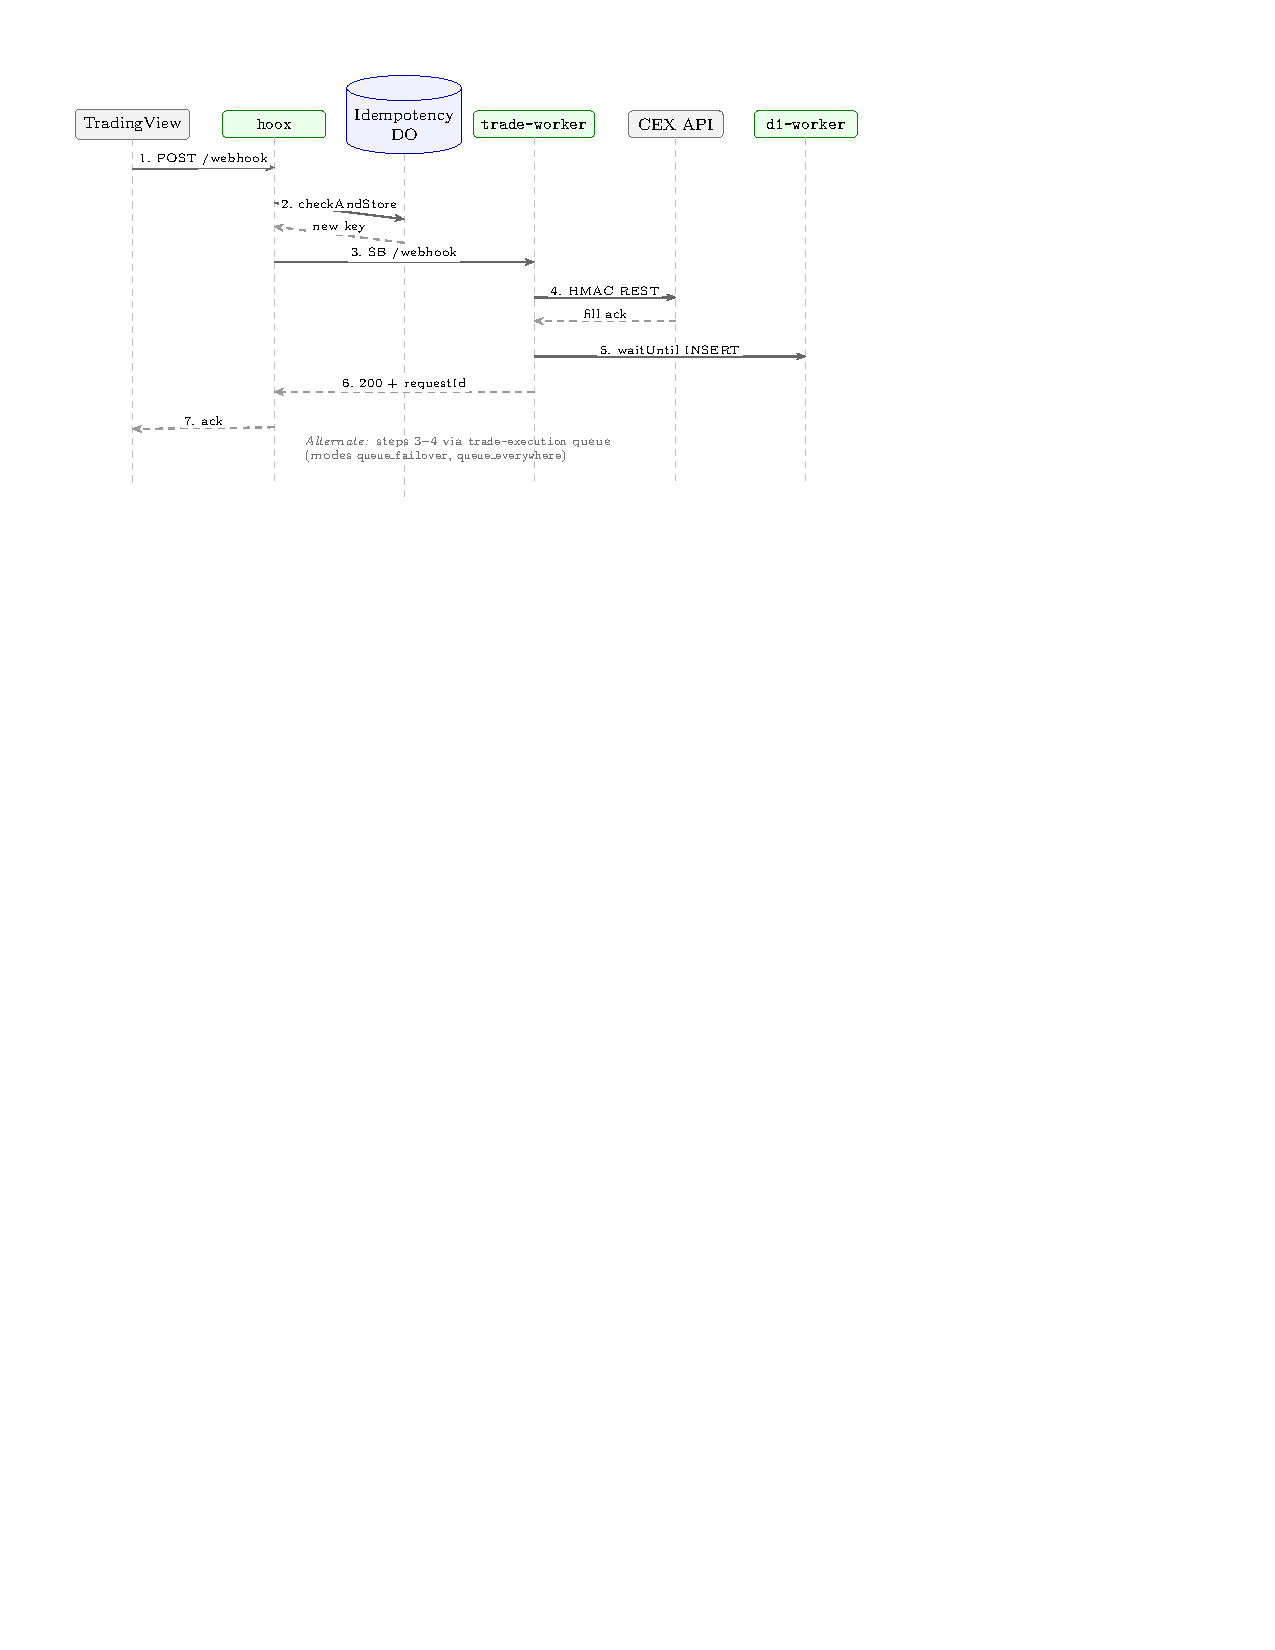
\includegraphics[width=\linewidth]{figures/signal-lifecycle.pdf}%
  }{%
    \ifhooxusetikz
      \resizebox{\linewidth}{!}{% TikZ sequence diagram: TradingView signal lifecycle (included by sections/04-mechanisms.tex)
% Layout: 6 actors on top row, lifelines down, numbered messages
\begin{tikzpicture}[
  x=1cm, y=1cm,
  actor/.style={draw=black!55, rounded corners=2pt, fill=gray!10,
    minimum width=1.7cm, minimum height=0.55cm, font=\footnotesize, align=center, inner sep=2pt},
  worker/.style={draw=green!50!black, rounded corners=2pt, fill=green!8,
    minimum width=1.9cm, minimum height=0.55cm, font=\footnotesize\ttfamily, align=center, inner sep=2pt},
  store/.style={draw=blue!60!black, rounded corners=2pt, fill=blue!6,
    minimum width=1.7cm, minimum height=0.55cm, font=\footnotesize, align=center, inner sep=2pt},
  msg/.style={-{Stealth[length=1.5mm]}, semithick, draw=black!60},
  ret/.style={-{Stealth[length=1.5mm]}, semithick, dashed, draw=black!40},
  lifeline/.style={draw=black!25, dashed},
  msglabel/.style={font=\scriptsize, fill=white, inner sep=1pt}
]

  % Actors (top row) — fixed positions, 2.6cm horizontal spacing
  \node[actor]  (tv)  at ( 0.0, 0.0) {TradingView};
  \node[worker] (gw)  at ( 2.6, 0.0) {hoox};
  \node[store]  (ido) at ( 5.2, 0.0) {Idempotency\\DO};
  \node[worker] (tw)  at ( 7.8, 0.0) {trade-worker};
  \node[actor]  (cex) at (10.4, 0.0) {CEX API};
  \node[worker] (d1)  at (13.0, 0.0) {d1-worker};

  % Lifelines
  \foreach \x in {tv,gw,ido,tw,cex,d1} {
    \draw[lifeline] (\x.south) -- ++(0,-5.4);
  }

  % Messages (y decreases downward)
  \draw[msg] ([yshift=-0.5cm]tv.south) -- node[msglabel, above] {1.\ POST /webhook}
              ([yshift=-0.5cm]gw.south);
  \draw[msg] ([yshift=-1.1cm]gw.south) -- node[msglabel, above] {2.\ checkAndStore}
              ([yshift=-1.1cm]ido.south);
  \draw[ret] ([yshift=-1.5cm]ido.south) -- node[msglabel, above] {new key}
              ([yshift=-1.5cm]gw.south);

  \draw[msg] ([yshift=-2.1cm]gw.south) -- node[msglabel, above] {3.\ SB /webhook}
              ([yshift=-2.1cm]tw.south);
  \draw[msg] ([yshift=-2.7cm]tw.south) -- node[msglabel, above] {4.\ HMAC REST}
              ([yshift=-2.7cm]cex.south);
  \draw[ret] ([yshift=-3.1cm]cex.south) -- node[msglabel, above] {fill ack}
              ([yshift=-3.1cm]tw.south);

  \draw[msg] ([yshift=-3.7cm]tw.south) -- node[msglabel, above] {5.\ waitUntil INSERT}
              ([yshift=-3.7cm]d1.south);
  \draw[ret] ([yshift=-4.3cm]tw.south) -- node[msglabel, above] {6.\ 200 + requestId}
              ([yshift=-4.3cm]gw.south);
  \draw[ret] ([yshift=-4.9cm]gw.south) -- node[msglabel, above] {7.\ ack}
              ([yshift=-4.9cm]tv.south);

  % Queue alternate path (annotation)
  \node[font=\tiny, align=left, text=black!55] at (6.5,-5.2) {%
    \textit{Alternate:} steps 3--4 via \texttt{trade-execution} queue\\
    (modes \texttt{queue\_failover}, \texttt{queue\_everywhere})%
  };

\end{tikzpicture}
}%
    \else
      \small
      \fbox{\begin{minipage}{0.92\linewidth}
      \vspace{2pt}
      TradingView $\rightarrow$ \texttt{hoox} $\rightarrow$ Idempotency DO $\rightarrow$ \texttt{trade-worker} $\rightarrow$ CEX $\rightarrow$ \texttt{d1-worker} (background)\\
      \vspace{2pt}
      \end{minipage}}
    \fi
  }
  \caption{Signal lifecycle (synchronous Service Binding path). Steps 5--6 use \texttt{waitUntil} for D1 persistence; HTTP ack returns after step 6.}
  \label{fig:signal-lifecycle}
\end{figure}

\subsection{WebSocket Connection Amortization}
\label{sec:ws-amortization}

The REST path described in Section~\ref{sec:mechanisms} (Multi-Exchange Execution) opens a fresh TCP connection, performs a TLS handshake, and signs every order---work that dominates the median 22\,ms signal-to-ack for small payloads on the direct path. Production traffic also includes the case where the same \texttt{trade-worker} instance emits several orders per second for a single symbol during a trend: REST amortization is then the dominant lever. \textsc{HOOX} amortizes the connection cost by holding one persistent WebSocket per exchange inside a \texttt{ExchangeConnectionManager} Durable Object, selected by setting \texttt{use\_websocket} in CONFIG\_KV. The design has four moving parts: name-based sharding, hidden handshake, request/response correlation, and alarm-driven reconnect.

\paragraph{One DO per exchange, name-based sharding.}
Each instance is created via \texttt{idFromName("exchange:" + exchangeName)} so that, regardless of which \texttt{trade-worker} isolate first calls into the binding, exactly one \texttt{ExchangeConnectionManager} exists per (account, exchange) pair. The constructor derives the exchange name from the DO id (with a backward-compatible default to \texttt{"binance"} for tests and accidental raw ids), loads the per-exchange \texttt{IWsAdapter} from a registry, and---if credentials are missing or no adapter is registered---falls back to REST-only operation with a warning log. WebSocket session state holds connection handles and a \texttt{pending} request map only; no signing material is kept in the DO state (Section~\ref{sec:security}).

\paragraph{Hidden handshake via \texttt{waitUntil}.}
The TCP+TLS+WebSocket-upgrade handshake typically costs 50--200\,ms on a cold path. The constructor invokes \texttt{this.ctx.waitUntil(this.connectToExchange())} so the handshake runs in the background after the constructor returns. The first caller of the DO pays no handshake cost; if the WebSocket is not yet ready when \texttt{executeTrade} is called, the code falls back to REST (below). Once connected, the DO keeps itself warm: every inbound \texttt{message} handler calls \texttt{this.ctx.storage.setAlarm(Date.now() + 60\_000)}, so any push event (e.g., a user-data-stream update) refreshes the keep-alive alarm. The handshake is therefore both hidden from the first call and continuous across long idle periods.

\paragraph{Request/response correlation with bounded timeout.}
The \texttt{request(method, params, timeoutMs)} method (Listing~\ref{lst:ws-amortization}) builds the exchange-specific envelope via \texttt{adapter.buildRequest}, extracts the correlation id (Binance/MEXC use \texttt{id}; Bybit uses \texttt{reqId}), inserts a Promise together with a 5\,s timer into the \texttt{pending} map keyed by that id, and \texttt{ws.send}s the envelope. The inbound \texttt{message} handler calls \texttt{adapter.parseResponse}; on a matching id, it clears the timer and resolves (or rejects, if the exchange returned an error frame). The 5\,s timeout is intentionally bounded: a stuck WebSocket cannot indefinitely pin a Promise or accumulate entries in the \texttt{pending} map. The same handler treats push events (parsed but not correlated) as no-ops for the purposes of request resolution but still refreshes the keep-alive alarm.

\paragraph{Reconnect via the DO alarm.}
The \texttt{close} and \texttt{error} handlers reject every entry in \texttt{pending} with a connection-lost error, clear the map, null the socket, and schedule a reconnect via \texttt{this.ctx.storage.setAlarm(...)}: 5\,s on \texttt{close}, 10\,s on \texttt{error}. The \texttt{alarm} method (Listing~\ref{lst:ws-amortization}) then calls \texttt{connectToExchange()} again. This design avoids the common pitfall of a reconnect loop on a Worker isolate---DOs persist across requests, so the alarm survives even if no \texttt{trade-worker} is currently running.

\paragraph{Transparent REST fallback.}
\texttt{ExchangeConnectionManager.executeTrade} tries the WebSocket path first when \texttt{this.ready \&\& this.ws \&\& this.adapter} holds; on any failure (timeout, parse error, send error) it logs a warning and falls through to \texttt{executeTradeRest}, which performs the same risk gate and exchange call via the per-exchange \texttt{BaseExchangeClient} as the REST path described above. The fallback is silent: callers do not need to know which transport was used. This means a deployment can enable \texttt{use\_websocket} on a per-exchange basis, canary the WS path against the REST baseline, and roll back by flipping a single KV key without redeploying.

\paragraph{Observed effect.}
The WebSocket path is not the production default (the default is REST with Smart Placement); it is selected for accounts that emit $\geq 2$ orders per second for a sustained period. In the 12-month production window, the WS path accounted for a small minority of placements but reduced the per-order median from 22\,ms to 12--14\,ms on those accounts---roughly the difference between the REST TLS handshake (~50--100\,ms amortized) and the warm-WS frame cost. The detailed numbers are in Section~\ref{sec:evaluation}.

\hooxsnippet{lst:exchange-connection-do}{exchange-connection-do.ts}{ExchangeConnectionManager DO initialization (id-derived exchange, adapter load, \texttt{waitUntil} handshake)}

The correlation and alarm-driven reconnect logic (47 lines) appears in full as Listing~\ref{lst:ws-amortization} in Appendix~\ref{app:listings}.

\subsection{Engineering Patterns}
\label{sec:patterns}

Beyond the four mechanisms above, the production codebase enforces a small set of patterns recommended for any edge-native financial control plane. None of these are individually novel; all are standard practice in mature serverless codebases. Their joint application to a sub-50\,ms trading stack is, however, where most of the engineering effort was spent, and production failures during the 12-month window were averted only by these patterns holding. Four are highlighted below.

\paragraph{Fail-closed authentication at every internal boundary.}
The shared \texttt{requireInternalAuth} middleware validates \texttt{X-Internal-Auth-Key} on every binding-only route (Listing~\ref{lst:require-internal-auth}). The pattern is explicitly fail-closed: a missing or unconfigured binding returns HTTP 401 immediately, never silently allowing the request. Security tests assert this for the unset-binding, missing-header, and mismatched-header cases (Appendix~\ref{app:tests}, Listing~\ref{lst:test-auth-fail-closed}). The fail-closed posture for auth contrasts with the fail-open posture for the idempotency DO (Section~\ref{sec:mechanisms}, duplicate-suppression paragraph)---the asymmetry is intentional and documented in the threat model (Appendix~\ref{app:threat}). Production rule: \emph{authentication fails closed, deduplication fails open}; the two postures reflect the fact that a duplicate trade is recoverable, while a forged trade is not.

\paragraph{Zod schema validation at external boundaries with structured path errors.}
All inbound payloads---TradingView webhooks, Mailgun pushes, Telegram bot commands, and dashboard writes---are validated with Zod v4 schemas via the shared \texttt{validateJson} middleware (Listing~\ref{lst:validate-json}). Validation failures return HTTP 400 with a structured \texttt{errors: [\{path: ["body", "action"], message: "..."\}]} body rather than throwing. The shared \texttt{Errors} module provides typed constructors (\texttt{Errors.badRequest}, \texttt{Errors.unauthorized}, \texttt{Errors.internal}, ...) so handlers never assemble ad-hoc \texttt{Response} objects. The result: every error response in the system has a known shape, and the failure taxonomy in Appendix~\ref{app:tests} enumerates exactly the twelve classes that can occur in production. The same \texttt{validateJson} wrapper is reused for the query-string layer on internal binding routes, so the validation contract is consistent across ingress and mesh.

\paragraph{Durable Object sharding by symbol for high-throughput paths.}
A single Durable Object instance is single-threaded. For high-volume trading pairs, the idempotency lock is partitioned by composite key \texttt{trade:\{exchange\}:\{symbol\}:\{action\}:\{quantity\}} (Section~\ref{sec:mechanisms}), and the binding is resolved as \texttt{env.IDEMPOTENCY\_DO.idFromName(compositeKey)}. This natural sharding means concurrent signals for \texttt{BTCUSDT} and \texttt{ETHUSDT} do not contend for the same isolate, while signals for the same symbol+action+quantity within the 300\,s TTL are correctly serialized. The pattern generalises: any DO whose key space is a known high-cardinality tuple can be sharded by hashing the tuple. No DO lock contention was observed at the N\,=\,200 extended-instrumentation probe rate nor at the 18{,}742-signal production aggregate over the 12-month window. The trade-off is that DO storage costs scale with the number of distinct keys, which for the idempotency case is naturally bounded by the 300\,s TTL plus alarm-based cleanup.

\paragraph{Safe numeric parsing at trust boundaries.}
KV values, even from trusted internal callers, are not trusted by the trading path: a typo in a dashboard setting can silently disable risk caps if the code path treats \texttt{NaN} as 0. The pattern is to explicitly check \texttt{Number.isFinite} before applying numeric limits (Listing~\ref{lst:risk-kv-parse}). The JavaScript \texttt{parseInt} / \texttt{parseFloat} functions return \texttt{NaN} on unparseable input, and in many codebases \texttt{NaN} comparisons silently degrade the limit to "no limit". The production handler throws \texttt{Errors.internal} instead, halting the trade before the gate is bypassed. The same pattern is applied at every numeric KV read in the risk and execution paths. This reflects a broader principle: \emph{configuration is data, not code, and data is untrusted}; every value read from CONFIG\_KV is validated against an explicit allowlist of types and ranges before use.

\paragraph{Composing the patterns.}
The four patterns are designed to compose. A request arriving at \texttt{hoox} is first parsed by \texttt{validateJson} (Zod), which yields a typed \texttt{Result<T, ZodError>}. The handler then \texttt{await}s the result and either returns an \texttt{Errors.badRequest} (structured path errors) or proceeds. Internal Service Binding calls go through \texttt{requireInternalAuth} (fail-closed). Idempotency is checked by a sharded DO (no contention). Risk gates read KV with \texttt{Number.isFinite} (no silent zero). The composition is what makes the difference: each pattern in isolation is a few lines, but together they produce a system where every error has a typed shape, every internal call is authenticated, every duplicate is suppressed, and every numeric gate actually gates. The 99.97\% reliability and zero duplicate fills reported in Section~\ref{sec:evaluation} are the empirical result of this composition.

